\documentclass[a4paper, 12pt, oneside]{extbook}
\usepackage[T1]{fontenc}
\usepackage[utf8]{inputenc}
\usepackage{geometry}
\usepackage{courier}
\usepackage{xcolor}
\usepackage{listings}
\lstset{language=bash}

\usepackage[bookmarks]{hyperref}
\newgeometry{
left=   1.5 in,
bottom= 1.5 in,
right=  1 in,
top=    1 in
}



\usepackage{fancyhdr}

% Grafica
\usepackage{graphics}
\graphicspath{{img/}}

% Package usati per il frontespizio
\usepackage{tikz}
\usepackage{pgf-pie}
\usepackage{pgfplots}
\pgfplotsset{width=7cm,compat=1.8}
\usetikzlibrary{patterns}


\setlength\headheight{44.2pt}
%Page Style
\usepackage{setspace}
%\setstretch{2.5} 
%\doublespace

%\cfoot{\thepage}
\lhead[]{}
\rhead[]{\leftmark}

\pagestyle{fancy}{
\lhead{
\includegraphics[scale=0.3]{img/logo/hlogo.png}}
\rhead{\footnotesize{Elaborato Network Security}}
}



\begin{document}

%\maketitle
\begin{titlepage}
\thispagestyle{empty}
\raggedright % Allinea a sinistra

\begin{tikzpicture}
\node[anchor=south west] at (4,0) {
\includegraphics[scale=0.75]{img/logo/logo_copertina_1}};
\node[anchor=south west] at (0,1.5) {
\includegraphics{img/logo/logo_copertina_2}};
\node[anchor=south west] at (0,0.5) {\textsf{Scuola Politecnica e delle Scienze di Base}};
\node[anchor=south west] at (0,0) {\textsf{Corso di Laurea Magistrale in Ingegneria Informatica}};
\end{tikzpicture}

\vfill

{\textbf{\textit{\LARGE Elaborato di Network Security}}}
\\[1cm]
{\large Anno Accademico 2022/2023}

\vfill


\begin{table}[h]
{\raggedright}

\textbf{Christian Marescalco}

\textbf{matr. M63001367}

\textbf{Antonio Avolio}

\textbf{matr. M63001352}
\end{table}

\end{titlepage}
\frontmatter

{\setstretch{1.5}
\tableofcontents
}

% stile per comandi bash
\lstdefinestyle{DOS}
{
  language=bash,
  basicstyle=\color{black},
    % backgroundcolor=\color{black},
    % basicstyle=\color{white}\fontfamily{ttfamily},
  showspaces=false,
  showstringspaces=false,
}
\linespread{1}
\onehalfspacing

\mainmatter




\chapter{Introduction}
In this paper an example of espionage attack will be emulated. 
The attacker Bob is infiltrated in a company's local network and exploits vulnerabilities to gain privileged access to the entire system.
The vulnerabilities concern: a company's local web server that makes insecure requests to the database; the employee Tom's vulnerable computer.
The entire example is compliant with Docker Security Playground (DSP), through which it can be emulated.
\section{Network Configuration}
\begin{center}
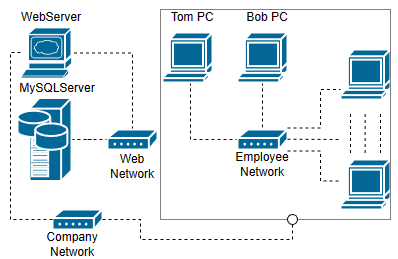
\includegraphics[scale=1]{../Image/network.PNG}
\end{center}
Sql Network: 
\begin{itemize}
  \item Web Server: it hosts a simple NodeJS website.
  \item MySQL Server: it stores sensitive information of the company
\end{itemize} 
Employee Network: 
\begin{itemize}
  \item BobPC: it represents the attacker host.
  \item TomPC: it represents the target host.
\end{itemize} 
Company Network: it connects all the employees to the company web service.


\chapter{Footprinting}
The footprinting phase involves gathering information in the network regarding the target, in our case the organization and its members.
\newline In this scenario, the attacker already knows information regarding the company and has managed to connect to the target local network.
\newline Through the \textit{ifconfig} tool, he discovers the subnets to which he is connected: Employee Network, Company Network.
\newline ifconfig screen
\newline Using the \textit{nmap} tool, the attacker discovers the topology of the various subnets within the organization, identifying the IPs of potential target nodes.
\begin{center}
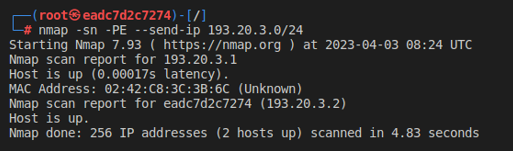
\includegraphics[scale=1]{../Image/footprinting_company_network.png}
\end{center}
\begin{center}
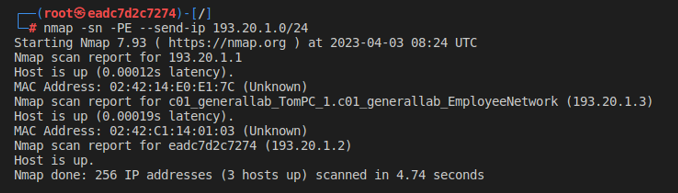
\includegraphics[scale=0.76]{../Image/footprinting_employee_network.png}
\end{center}
From the top scan of the IP range 193.20.3.0/24, Bob found out one host up at 193.20.3.1 and its MAC Address. On the other subnet 193.20.1.0/24, there is another host up with the address 193.20.1.2.

\chapter{Scanning}
In this phase, the attacker explores the entire network perimeter to gather information about 
the target network in order to identify potential vulnerabilities and weak points that can be exploited.  
\newline The scanning phase typically involves a combination of active and passive scanning methods. Active scanning involves 
sending probe packets or requests to target systems to elicit a response, while passive scanning involves observing and analyzing network traffic without actually engaging with the target systems. 
This is typically done using various scanning tools and techniques, including \textbf{\textit{Nmap}}: Network Mapper, a versatile and powerful tool with a range of options and features. 
Here are some of the main options:
\begin{itemize}
  \item Host Discovery: This option is used to discover hosts on a network. Nmap can identify active hosts, as well as those that are currently offline.
  \item Port Scanning: Port scanning is one of the most popular features of Nmap. It can be used to identify open ports on a target system, and even detect hidden ports and services.
  \item Service and Version Detection: This option is used to identify the services and versions of software running on the target system. This information can be useful in identifying vulnerabilities and weaknesses.
  \item Operating System Detection: Nmap can also be used to identify the operating system running on the target system. This information can be helpful in identifying potential attack vectors.
  \item Scripting Engine: Nmap has a powerful scripting engine that allows users to write and execute custom scripts. This feature can be used to automate tasks, customize scans, and extend the functionality of Nmap.
\end{itemize} 
These are just a few of the main options available in Nmap. Other features include traceroute, firewall detection, and performance tuning options.
It has a number of flags or options that can be used to customize and fine-tune its scanning behaviour.
\newline Here are some commonly used flag options:
\begin{itemize}
  \item \textbf{-sS}: This flag specifies the type of scan to be performed, in this case a SYN scan.
  \item \textbf{-sT}: This flag specifies a TCP connect scan, where Nmap attempts to establish a full TCP connection with the target ports.
  \item \textbf{-sU}: This flag specifies a UDP scan, where Nmap sends UDP packets to the target ports and listens for responses.
  \item \textbf{-sC}: This flag specifies a scan usiong the default set of scripts. Some of the scripts in this category are considered intrusive.
  \item \textbf{-O}: This flag enables operating system detection, allowing Nmap to identify the operating system running on the target system.
\end{itemize}
The attacker Bob exploits the following nmap command to discover open services on the target host 193.20.3.1:
\begin{center}
  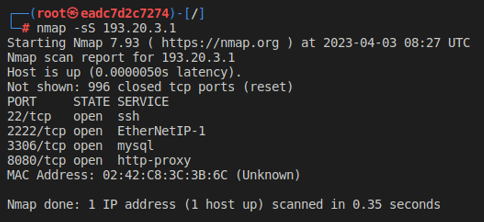
\includegraphics[scale=0.76]{../Image/scanning_company_ss.PNG}
\end{center}
From the scan report, there are multiple open ports: \textit{http} on 8080, \textit{mysql} on 3306 and \textit{ssh} on 22. The attacker can assume that the target host 193.20.3.1 is a Web Server.
\newline Then, he does the same for the node on the other subnet:
\begin{center}
  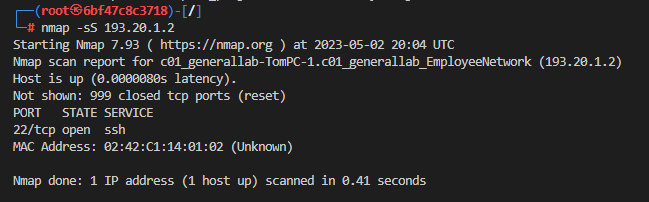
\includegraphics[scale=0.76]{../Image/scanning_employee_ss.PNG}
\end{center}
From the scan report, there is only an open SSH 22/Tcp port.

\chapter{Enumeration}
The primary goal of the enumeration phase is to identify potential targets for further exploitation and gain a deeper understanding of the target network's structure and architecture.
After discovering the potential access points on the hosts, it is necessary to reveal other information regarding the active services on the detected ports. In the enumeration phase,
active connections are created towards the target services by using the nmap tool with appropriate flags. This phase is more dangerous and traceable than the previous techniques because it requires an higher level of intrusiveness.
\newline The objective of this phase is the service fingerprinting, i.e. the detection of the specific version and implementation of the service through an analysis of the service behaviour. 
\newline The attacker uses the nmap flag -sV, which compares answers obtained with a service fingerprint database, to determine services version on the Web Server:
\begin{center}
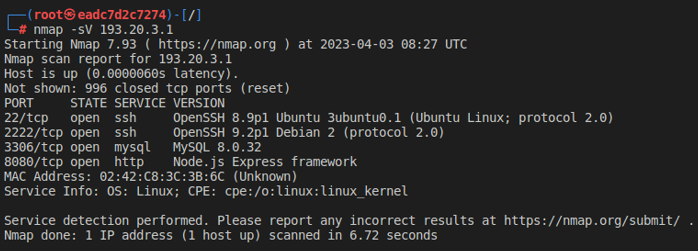
\includegraphics[scale=0.76]{../Image/enumeration_company_sv.PNG}
\end{center}
The attacker grabs information about the Web Server: it is implemented with NodeJS and has a connection with a mySQL Database. Then, he does the same for the Employee computer:
\begin{center}
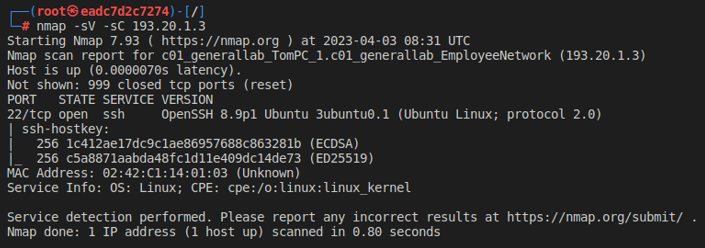
\includegraphics[scale=0.76]{../Image/enumeration_tom_sv.PNG}
\end{center}
On the other host, nmap determines that: the ssh service is implemented with a specific version of OpenSSH and the OS family is Ubuntu Linux. 
\newline With the tool \textit{curl} or \textit{wget}, the attacker can get information about the website pages. In a real case scenario, it is better to map the entire site with \textit{Dirbuster} or an analogous tool.
\begin{center}
  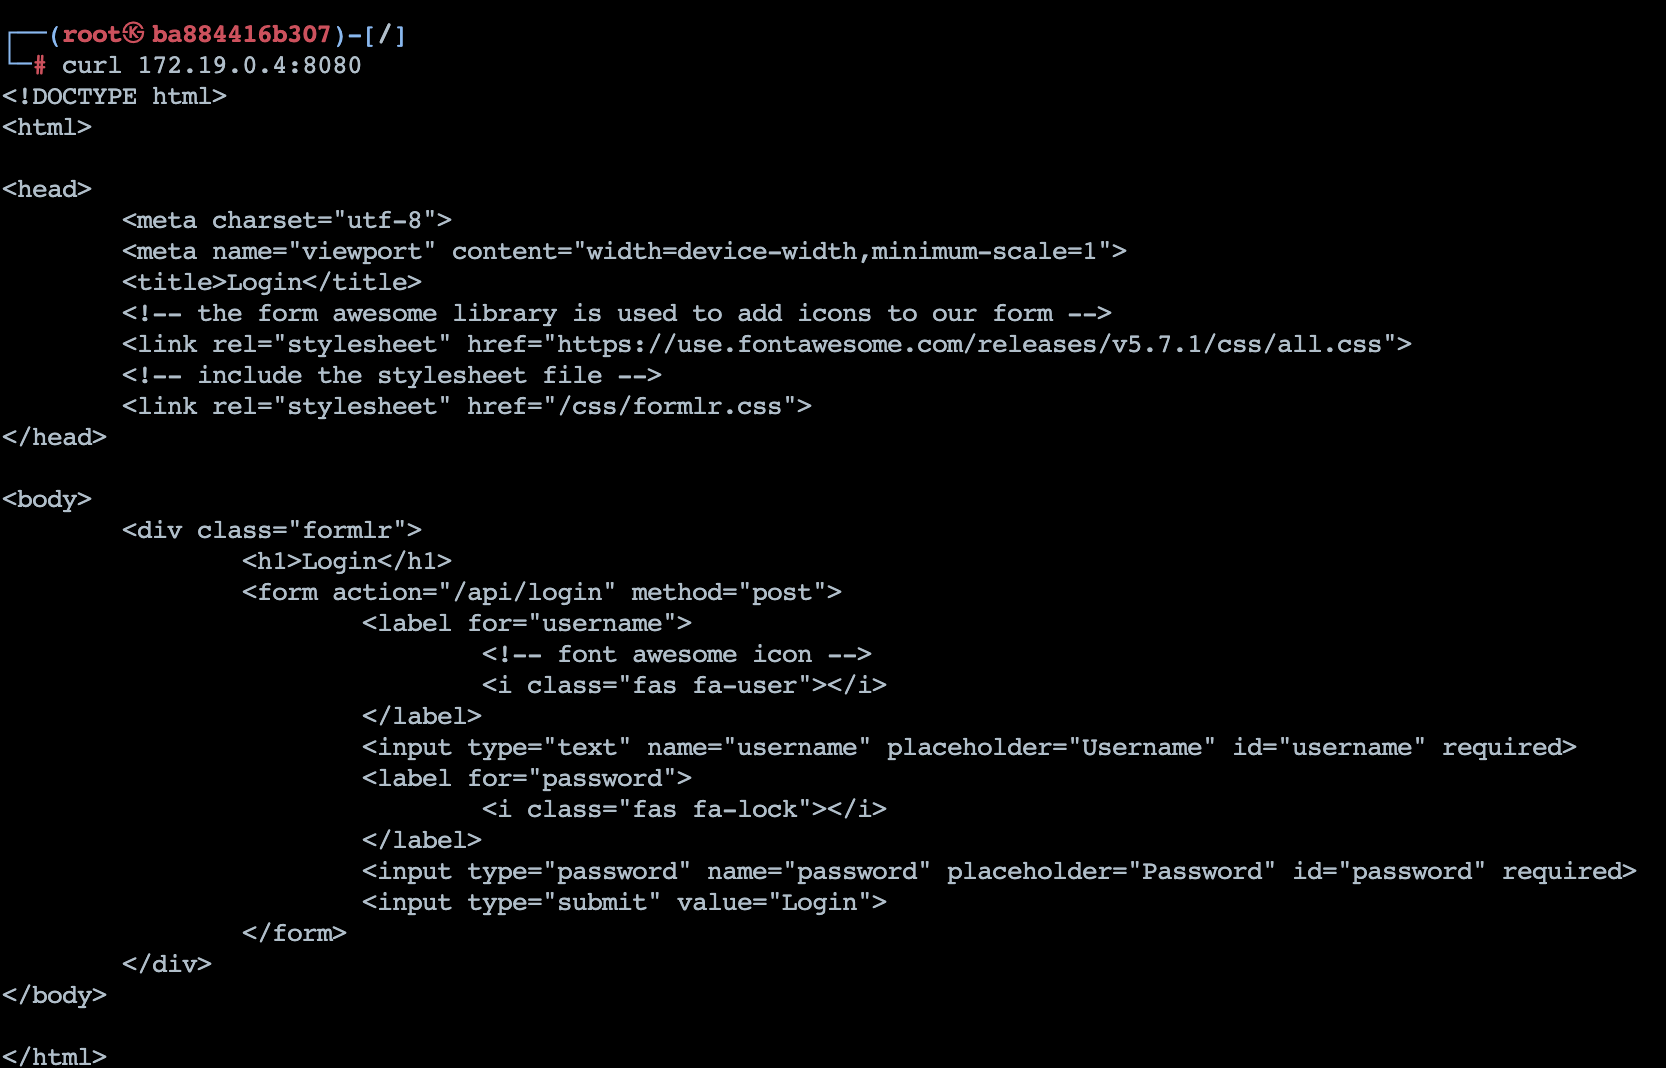
\includegraphics[scale=0.66]{../Image/webserver_curl.PNG}
\end{center}
From the last command, the attacker Bob discovers a login page that may be exploited.
Once vulnerabilities are identified, the attacker can move on to the next phase of the attack, the exploitation phase.

\chapter{Exploitation}
The exploitation phase has the objective of gaining access to the target system and obtaining privileged information, such as usernames, passwords, and other sensitive data. 
Attackers may use various methods to exploit vulnerabilities in the target system, including:
\begin{enumerate}
  \item Social engineering: Attackers may use social tactics to trick users into revealing sensitive information or clicking on malicious links that can install malware or grant unauthorized access to the target system.
  \item Malware: Attackers may use malware, such as viruses, Trojans, or worms, to exploit vulnerabilities in the target system and gain unauthorized access.
  \item Remote exploits: Attackers may use remote exploits to take advantage of vulnerabilities in network protocols or services, such as TCP/IP or HTTP, to gain unauthorized access to the target system.
  \item Exploit kits: Attackers may use exploit kits, which are pre-packaged sets of tools and exploits, to automate the process of finding and exploiting vulnerabilities in the target system.
\end{enumerate}

In this case, the attacker Bob uses a mix of remote exploits to gain root access on the Employee PC.

\section{Sql Injection}
The attacker starts from the company web service by filling the login form with different combinations:

\begin{lstlisting}[style=DOS]
$ curl -X POST -d 'username=a&password=b' 193.20.3.1:8080
\end{lstlisting}
In this case, the website uses an url-encoded form, so the attacker can send the data as an url-encoded string. This one returns "Error value(s) missing".
\newline The attacker tries to tamper the form with another combination:
\begin{lstlisting}[style=DOS]
$ curl -X POST -d 'username=&password=b' 193.20.3.1:8080
\end{lstlisting}
which returns:
\begin{lstlisting}[style=DOS]
$ {"success":false,"response":"No user found","result":[]}
\end{lstlisting}
Lastly, the attacker can try to insert a payload with a MySQL Injection, that uses OR and the commenting syntax:
\begin{lstlisting}[style=DOS]
$ curl -X POST -d 'username=" OR 1<2; -- &password=b' \
$ 193.20.3.1:8080
\end{lstlisting}
which returns a list of credentials:
\begin{center}
  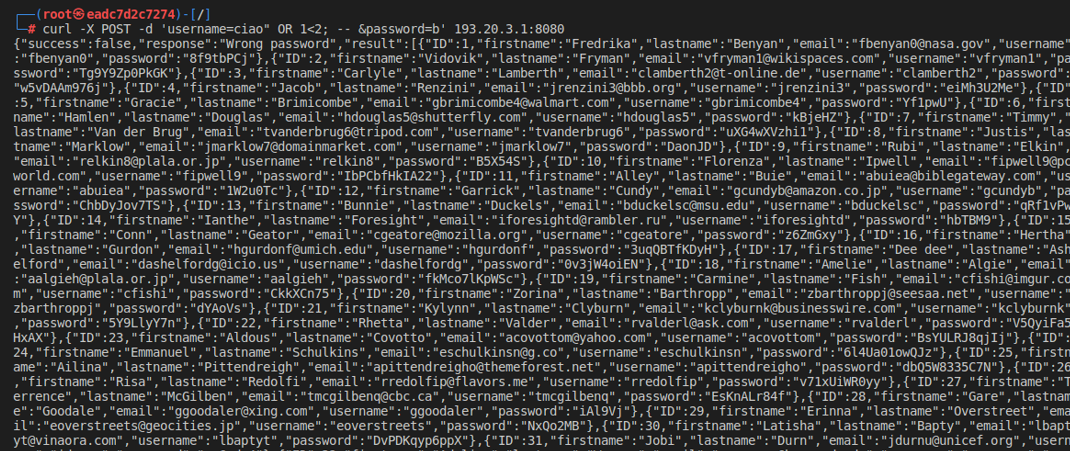
\includegraphics[scale=0.5]{../Image/webserver_sql.PNG}
\end{center}
including an entry related to the user Tom:
\begin{lstlisting}[style=DOS]
  username = tcasaccio1
  password = YLN1NrMdGN
\end{lstlisting}

\section{SSH Access}
Now, the attacker can access to the target machine which has an open SSH port:
\begin{lstlisting}[style=DOS]
$ ssh tcasaccio1@193.20.1.3
\end{lstlisting}

\section{Privilege escalation}
From the ssh entrypoint on TomPC, the attacker can trace Tom privileges on the machine 
and which files can be accessed with unnecessary privileges:
\begin{center}
  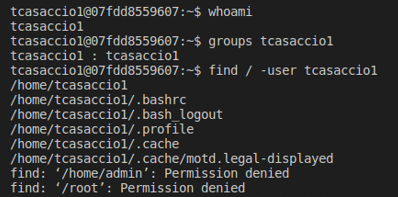
\includegraphics[scale=1]{../Image/privilege_escalation_whoami.PNG}
\end{center}
Although the user tcasaccio1 doesn't belong to sudo group, Bob can check  
/etc/passwd to trace all users on the PC: 
\begin{center}
  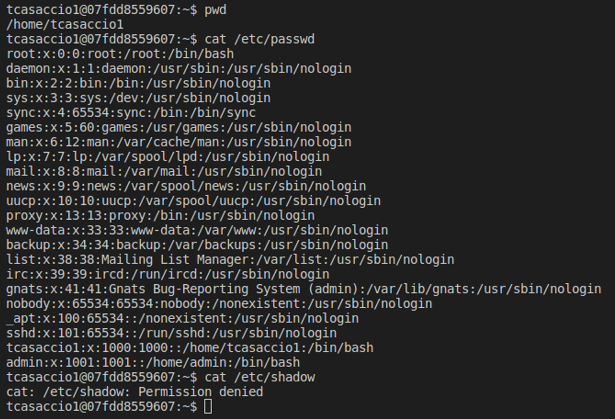
\includegraphics[scale=0.8]{../Image/privilege_escalation_passwd.PNG}
\end{center}
The attacker can't access to /etc/shadow, so he needs to find a workaround to gain elevated privileges. 
Firstly, he checks the SUID files.
\newline The Set User IDentity bit allows users to run executables with the file system permissions
of the executable's owner to perform a specific task, in this case with root privilege.
The SUID bit is normally represented as value 4 in the high-order octal digit of the file mode.
\newline So, by using the following command:
\begin{center}
  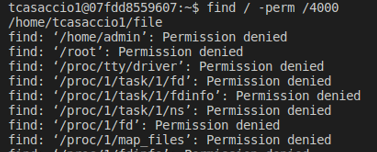
\includegraphics[scale=1]{../Image/privilege_escalation_suid.PNG}
\end{center}
the attacker is searching all files with the SUID bit set. In /home/tcasaccio1 there is a file with the SUID bit set,
so the attacker investigates the possible target directory:
\begin{center}
  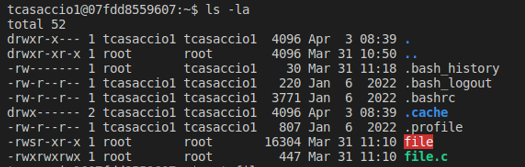
\includegraphics[scale=1]{../Image/privilege_escalation_suid2.PNG}
\end{center}
In the directory, there is also the source code of the target file:
\begin{center}
  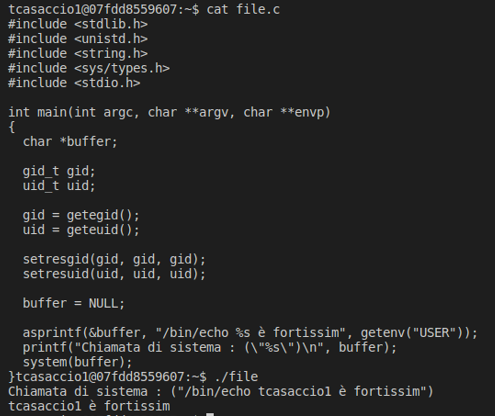
\includegraphics[scale=1]{../Image/privilege_escalation_program.PNG}
\end{center}
By inspection of the source code, the final system call instruction can be exploited to 
execute any command with root privileges, but the program doesn't allow the attacker to insert the 
payload by input. In this case, the workaround is the system call \textit{getenv}, which returns the environment 
variable specified as the function parameter. The attacker can modify the USER environment variable 
by creating an \textit{environment variable injection}:
\begin{lstlisting}[style=DOS]
$ export USER="; /bin/bash; echo ":tcasaccio1
\end{lstlisting}
obtaining this behaviour by the program:
\begin{center}
  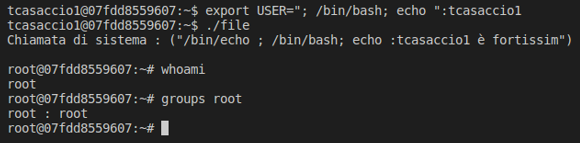
\includegraphics[scale=0.9]{../Image/privilege_escalation_exploit.PNG}
\end{center}
Finally, the attacker has obtainend root permissions on the machine.
To eliminate the footprints on the target machine, he deletes:
\begin{enumerate}
  \item the ssh log files in textit{/var/log/};
  \item the user tcasaccio1's bash history in \textit{/.bash\_history} to hide the exploitation process;
  \item the user root's bash history to hide any post-exploitation actions;
 \end{enumerate}

 \begin{center}
  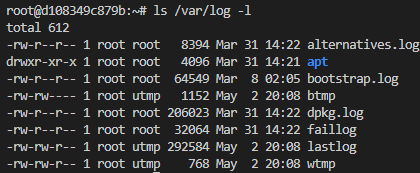
\includegraphics[scale=0.9]{../Image/elimination_traces.PNG}
\end{center}


\chapter{Countermeasures and defenses}
Some possible defenses to reduce or mitigate threats are divided based on the target asset.
\section*{SSH protocol}
\begin{itemize}
  \item Use a stronger key-based authentication instead of password-based authentication and configure the server to only allow key-based authentication.
  \item Change the default port 22 to prevent automated attacks from malicious actors.
 \end{itemize}

 \section*{Web Server}
\begin{itemize}
  \item Ensure that the login page is accessed over a secure connection using SSL/TLS encryption, this protects sensitive information, such as login credentials, from being intercepted by attackers.
  \item Use strong authentication such as multi-factor authentication or password policies, to ensure that only authorized users can access the web application.
  \item Use parameterized queries to protect against SQL injection attacks, which prevent attackers from injecting malicious code into SQL statements.
  \item Avoid disclosure of unnecessary log details about application logic errors, such as login failure attempts.
\end{itemize}

\section*{Setuid program}
\begin{itemize}
\item SUID bit should not be set to any program which lets you escape to the shell.
\item Perform input data sanitization and embed only predefined commands.
\item Never set SUID bit on any file editor/compiler/interpreter as an attacker can easily read/overwrite any files present on the system.
\end{itemize}

\end{document}